% A skeleton file for producing Computer Engineering reports
% https://kgcoe-git.rit.edu/jgm6496/KGCOEReport_template

\documentclass[CMPE]{../KGCOEReport}

% The following should be changed to represent your personal information
\newcommand{\classCode}{CMPE 260}  % 4 char code with number
\newcommand{\name}{Andrei Tumbar}
\newcommand{\LabSectionNum}{1}
\newcommand{\LabInstructor}{Moskal}    % The slash is to tell LaTeX that the period is between words
% not sentences so it spaces correctly. It won't appear in the
% final pdf
\newcommand{\TAs}{Jacob Meyerson\\Dennis Lam}
\newcommand{\LectureSectionNum}{1}
\newcommand{\LectureInstructor}{Cliver}
\newcommand{\exerciseNumber}{6}
\newcommand{\exerciseDescription}{Project 1 - Pipelined MIPS}
\newcommand{\dateDone}{May 1st}
\newcommand{\dateSubmitted}{May 3rd}

\usepackage{tikz}
\usepackage{circuitikz}
\usetikzlibrary{calc}
\usetikzlibrary{circuits.logic.IEC,calc}
\usepackage{multirow}
\usepackage{float}
\usepackage{lmodern}
\usepackage{siunitx}
\usepackage{subcaption}
\usepackage{graphicx}
\usepackage[usestackEOL]{stackengine}
\usepackage{scalerel}
\usepackage[T1]{fontenc}
\usepackage{amsmath}

\def\lbar#1{\ThisStyle{%
    \setbox0=\hbox{$\SavedStyle#1$}%
    \stackengine{2.2\LMpt}{$\SavedStyle#1$}{\rule{\wd0}{0.1\LMpt}}{O}{c}{F}{F}{S}%
}}

\DeclareFontFamily{U}{mathx}{\hyphenchar\font45}
\DeclareFontShape{U}{mathx}{m}{n}{ <-> mathx10 }{}
\DeclareSymbolFont{mathx}{U}{mathx}{m}{n}
\DeclareFontSubstitution{U}{mathx}{m}{n}
\DeclareMathAccent{\widebar}{\mathalpha}{mathx}{"73}

\makeatletter
\newcommand{\cwidebar}[2][0]{{\mathpalette\@cwidebar{{#1}{#2}}}}
\newcommand{\@cwidebar}[2]{\@cwideb@r{#1}#2}
\newcommand{\@cwideb@r}[3]{%
    \sbox\z@{$\m@th\mkern-#2mu#3\mkern#2mu$}%
    \widebar{\box\z@}%
}
\newcommand\currentcoordinate{\the\tikz@lastxsaved,\the\tikz@lastysaved}
\makeatother

\newcommand\decbin[9]{%
    \par\smallskip
    \makebox[3cm][r]{$#1$\ }\fbox{#2}\,\fbox{#3}\,\fbox{#4}\,\fbox{#5}\,\fbox{#6}\,\fbox{#7}\,\fbox{#8}\,\fbox{#9}\par}


\def\code#1{\texttt{#1}}

\begin{document}
    \maketitle
    \section*{Abstract}

    In this laboratory exercise, the pipelined MIPS was implemented by
    placing a register in-between the stages of the MIPS. The result of
    pipelining is that the clock period can be shorter but there is a
    delay when the instruction is loaded from instruction memory and when
    the result is ready for use. The programmer must be mindful of this
    delay and take it into account when writing the tests. To test the
    pipelined MIPS, two distinct programs were written: the first separately
    tests each valid instruction available on the processor. The second test
    will implement a fibonacci sequence and load the results into memory.

    \section*{Design Methodology}
	There are five main stages to the MIPS pipeline: Fetch, Decode/Register File,
	Execute, Memory, and Writeback. Signals between each stage are held between
	rising edge triggered flip-flops. This way their values may be propagated
	down the pipeline after each clock cycle.
    \\
    
    To easily test the process a set of scripts were created in Python. The
    first script, \code{mips\_asm.py} compiles a file written in standard MIPS
    assembly by encoding lines of assembly in hex. The second script will
    reprocess the compiled program into a format that VHDL can load 
    into instruction memory. The instruction memory was adapted to read lines
    of \code{.mem} files.
    \\
	
	Using the these two scripts to compile and initialize instruction memory,
	\code{part\_a.s} was implemented to test all of the separate instruction
	and \code{fib.s} was written to implement the fibonacci sequence. Separate
	registers were used to store each of the items in the fibanacci sequence
	up to $a_{10}$. Store instructions were performed after three clock cycles
	to write the data back to memory. The reason we have to wait three clock
	cycles is because there are four sets of registers and it takes a single
	cycle to load the instruction. To fill one of the dead cycles with a useful
	operation, the memory load from the previous item can be placed here. This
	means that there are two dead cycles per item in the sequence.
	\\
	
	To properly test that the results are correct and loaded into memory,
	after all of the sequence items are calculated and stored, we execute
	an instruction where to result is a special value that the testbench can
	verify. In this case the value \code{0xFFFFAB12} was chosen because its
	a large distinct value. Following the execution of this special instruction
	the output of each fibonacci item is loaded from memory and the test bench
	is able to verify the results by looking at the results of the instruction.
	A list was written in the testbench with the true first ten elements of the
	fibonacci sequence and verified against the results loaded from memory.
	
	\pagebreak
	
    \section*{Results \& Analysis}

    Test benches for part a and part b are shipped with expected outputs.
    There are self verifying by design with assertions placed throughout
    the simulation. A behavioural waveform was generated for part a to show
    the results. The part A testbench uses the lowest three registers for 
    inputs to test all operations.
	
	\begin{table}[H]
        \renewcommand{\arraystretch}{1.2}
        \setlength{\tabcolsep}{12pt}
        \caption{Input registers for Part A}
        \begin{center}
            \begin{tabular}{|c|c|c|}
                \hline
				Register & Value\\\hline

				% register   Operation     
				\code{r1} & \code{0xFFFFFEFE}\\\hline
				\code{r2} & \code{0xFFFFCECE}\\\hline
				\code{r3} & \code{0x8}\\\hline

            \end{tabular}
        \end{center}
        \label{tab:inputs}
    \end{table}

	Using these input values, all of the operations are tested. The
	following table will show the expected values for each of the ALU
	operations.
    
    
    \begin{table}[H]
        \renewcommand{\arraystretch}{1.2}
        \setlength{\tabcolsep}{12pt}
        \caption{Input registers for Part A}
        \begin{center}
            \begin{tabular}{|c|c|c|c|}
                \hline
				Operation & Operator 1 & Operator 2 & Output\\\hline

				\code{and} & \code{0x8} & \code{0xFFFFCECE} & \code{0x8}\\\hline
				\code{or} & \code{0x7} & \code{0xFFFFCECE} & \code{0xFFFFCECF}\\\hline
				\code{xor} & \code{0x7} & \code{0xFFFFCECE} & \code{0xFFFFCECF}\\\hline
				\code{multu} & \code{0xFEFE} & \code{0xCECE} & \code{0xCDFD9464}\\\hline
				\code{sll} & \code{0xFFFFFEFE} & \code{0x8} & \code{0xFFFEFE00}\\\hline
				\code{sra} & \code{0xFFFFCECE} & \code{0x8} & \code{0xFFFFFFCE}\\\hline
				\code{srl} & \code{0xFFFFCECE} & \code{0x8} & \code{0x00FFFFCE}\\\hline
				\code{sub} & \code{0xFFFFFEFE} & \code{0xFFFFCECE} & \code{0x3030}\\\hline
				\code{add} & \code{0xFFFFFEFE} & \code{0xFFFFCECE} & \code{0xFFFFCDCC}\\\hline

            \end{tabular}
        \end{center}
        \label{tab:operations}
    \end{table}

	Both the immediate and R-Type instructions for the relevant operations
	were tested. A waveform was created to show the output.
	
	\begin{figure}[h!]
        \centering
        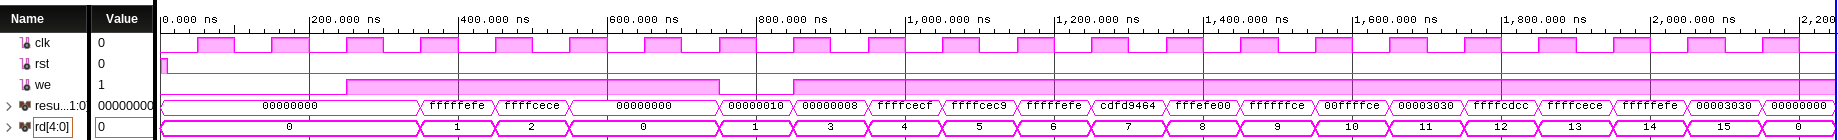
\includegraphics[width=\textwidth]{img/part_a_behav}
        \caption{Behavioural simulation of Part A}
        %! suppress = FigureNotReferenced
        \label{fig:demo1}
	\end{figure}

	The assertions placed in this test bench verify that the outputs
	are valid.
	\\
	
	Testing the fibonacci program is far simpler than the testbench in
	Part A. To test it simply verify that the output of the first then
	fibonacci numbers match the expected sequence:
	\code{0}, \code{1}, \code{1}, \code{2}, \code{3}, \code{5},
	\code{8}, \code{13}, \code{21}, \code{34}, \code{55}.
	
	A behavioural waveform was generated to verify the results. Outputs are
	formatted to decimal format to more easily see the results.
	
	\begin{figure}[h!]
        \centering
        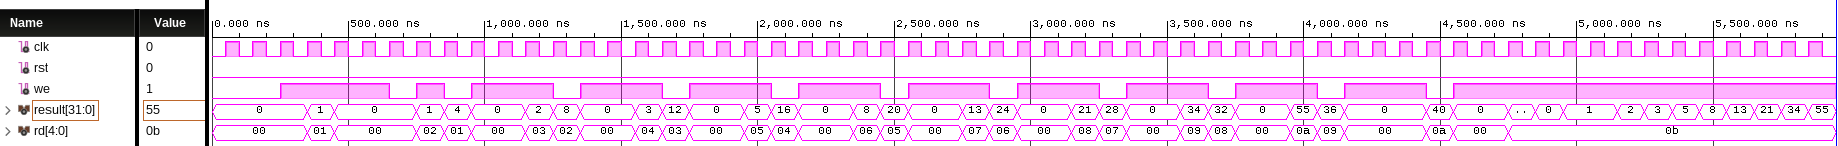
\includegraphics[width=\textwidth]{img/part_b_behav}
        \caption{Behavioural simulation of Part B}
        %! suppress = FigureNotReferenced
        \label{fig:fib_behav}
	\end{figure}

	Figure \ref{fig:fib_behav} and the fact that the simulation finished
	without tripping an shows the validity of the program and processor 
	implementation.

    \section*{Conclusion}
    
    This laboratory exercise finished the implementation of the pipelined
    MIPS processor. Testbenches written along with the assembly files
    helped verify the processor. While writing the pipelined MIPS, the
    it was deemed more efficient to get rid of the passthrough signals
    on the execute stage. The same functionality could be kept by
    passing signals through the pipeline instead. Looking at the results
    of the test programs and the waveforms generated by the testbenches,
    the implementation of the MIPS processor is a success.

    \pagebreak

    \section*{Demo results}
    \begin{figure}[h!]
        \centering
        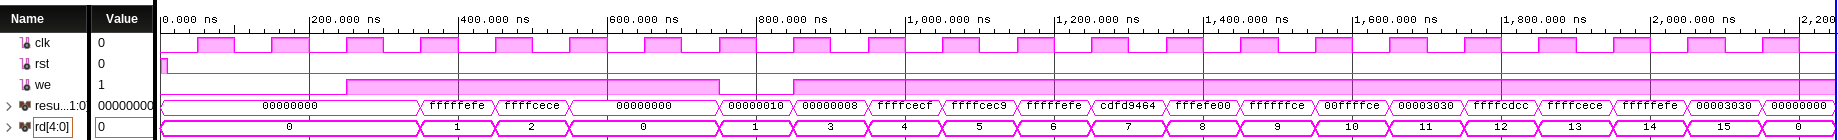
\includegraphics[width=\textwidth]{img/part_a_behav}
        \caption{Behavioural simulation of all instructions}
        %! suppress = FigureNotReferenced
        \label{fig:demo1}
	\end{figure}
    \begin{figure}[h!]
        \centering
        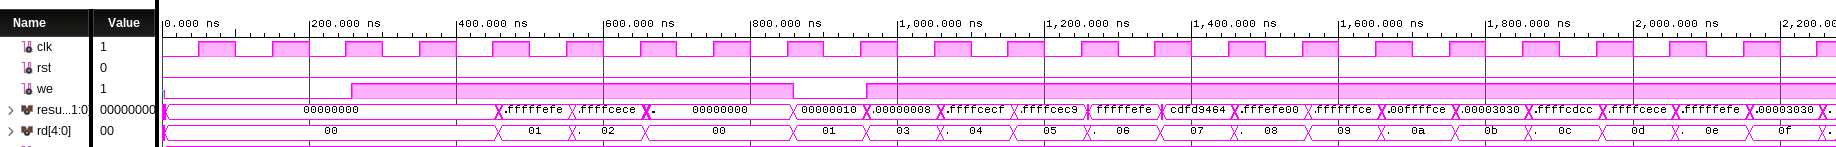
\includegraphics[width=\textwidth]{img/part_a_impl}
        \caption{Post-implementation timing simulation of all instructions}
        %! suppress = FigureNotReferenced
        \label{fig:demo1}
	\end{figure}
    \begin{figure}[h!]
        \centering
        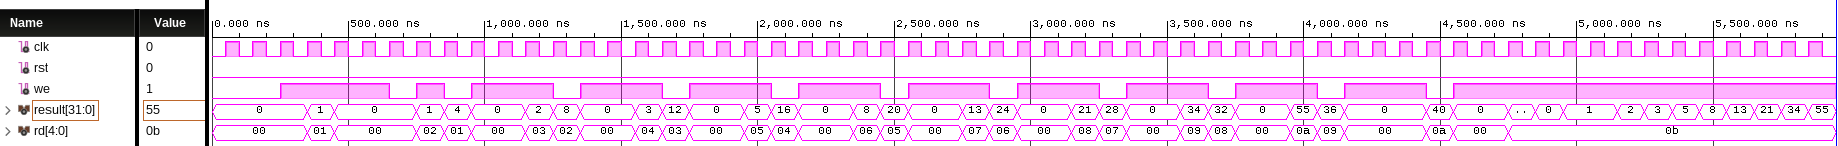
\includegraphics[width=\textwidth]{img/part_b_behav}
        \caption{Behavioural simulation of fibonacci sequence}
        %! suppress = FigureNotReferenced
        \label{fig:demo1}
	\end{figure}
    \begin{figure}[h!]
        \centering
        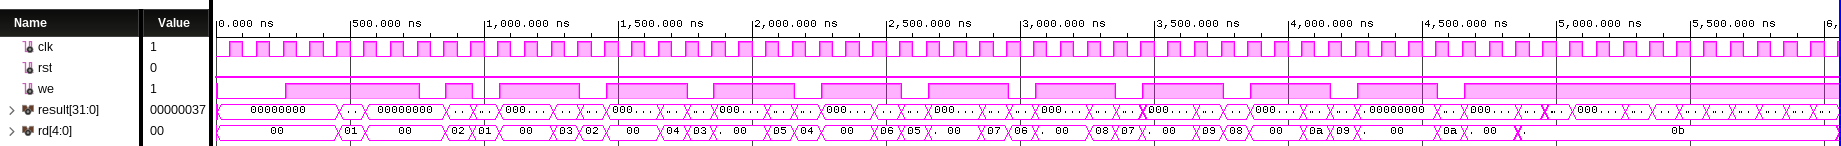
\includegraphics[width=\textwidth]{img/part_b_impl}
        \caption{Post-implementation timing simulation of fibonacci sequence}
        %! suppress = FigureNotReferenced
        \label{fig:demo1}
    \end{figure}

\end{document}